\documentclass[a4paper]{article}
\usepackage{student}

% Metadata
\date{\today}
\setmodule{ID5841: Quantum Computing Lab}
\setterm{Jul-Nov, 2022}

%-------------------------------%
% Other details
% TODO: Fill these
%-------------------------------%
\title{Assignment 1}
\setmembername{Chaganti Kamaraja Siddhartha}  % Fill group member names
\setmemberuid{EP20B012}  % Fill group member uids (same order)

%-------------------------------%
% Add / Delete commands and packages
% TODO: Add / Delete here as you need
%-------------------------------%
\usepackage{amsmath,amssymb,bm,pdfpages,graphicx,array}
\graphicspath{ {./1a/}{./1b/}{./2/}{./4/}{./5/} }
\newcommand{\KL}{\mathrm{KL}}
\newcommand{\R}{\mathbb{R}}
\newcommand{\E}{\mathbb{E}}
\newcommand{\T}{\top}

\newcommand{\expdist}[2]{%
        \normalfont{\textsc{Exp}}(#1, #2)%
    }
\newcommand{\expparam}{\bm \lambda}
\newcommand{\Expparam}{\bm \Lambda}
\newcommand{\natparam}{\bm \eta}
\newcommand{\Natparam}{\bm H}
\newcommand{\sufstat}{\bm u}

% Main document
\begin{document}
    % Add header
    \header{}

    % Use `answer` environment to add solutions
    % \begin{answer}[Question 1.1] for example starts an environment formatted
    % for Question 1.1
    \begin{answer}[Question 1 a]
        \subsection*{Circuit for 2 Fredkin gates on state 000}
        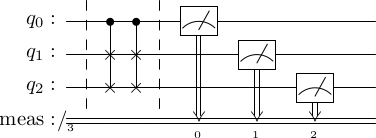
\includegraphics[scale = 0.5]{1a000.png}
        \subsection*{Output for input 000 is}
        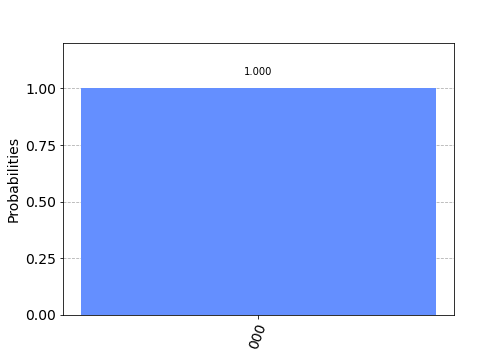
\includegraphics[scale = 0.5]{1a000-out.png}
        \subsection*{Circuit for 2 Fredkin gates on state 000}
        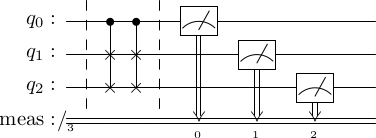
\includegraphics[scale = 0.5]{1a000.png}
        \subsection*{Output for input 000 is}
        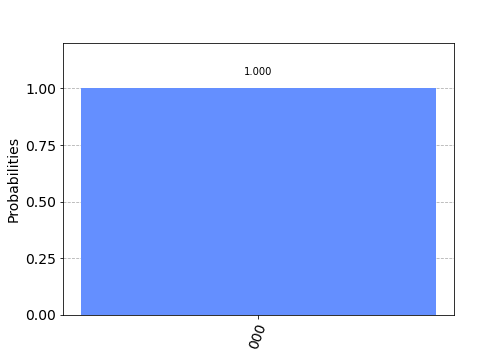
\includegraphics[scale = 0.5]{1a000-out.png}
        \subsection*{Circuit for 2 Fredkin gates on state 001}
        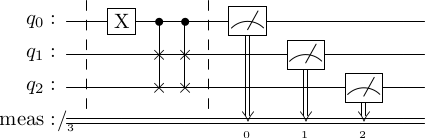
\includegraphics[scale = 0.5]{1a001.png}
        \subsection*{Output for input 001 is}
        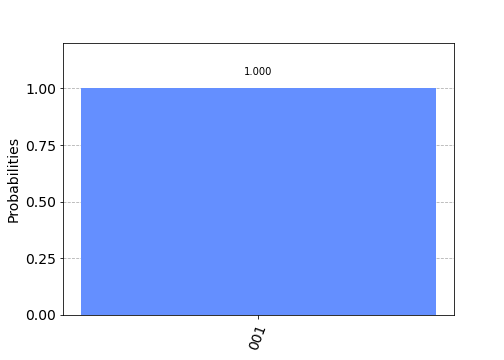
\includegraphics[scale = 0.5]{1a001-out.png}
        \subsection*{Circuit for 2 Fredkin gates on state 010}
        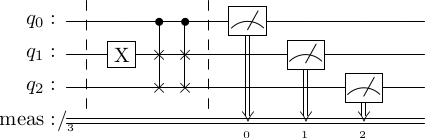
\includegraphics[scale = 0.5]{1a010.png}
        \subsection*{Output for input 010 is}
        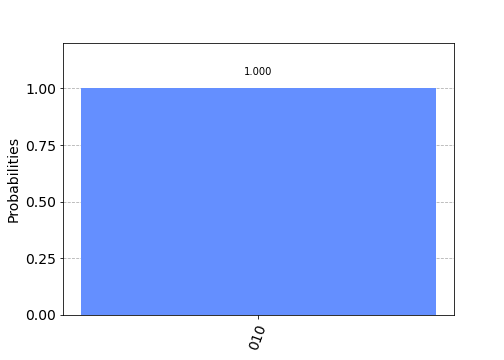
\includegraphics[scale = 0.5]{1a010-out.png}
        \subsection*{Circuit for 2 Fredkin gates on state 011}
        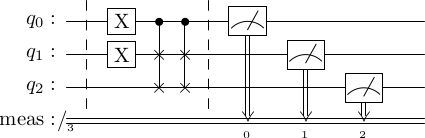
\includegraphics[scale = 0.5]{1a011.png}
        \subsection*{Output for input 011 is}
        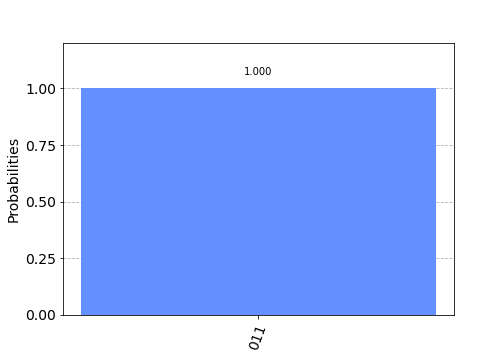
\includegraphics[scale = 0.5]{1a011-out.png}
        \subsection*{Circuit for 2 Fredkin gates on state 100}
        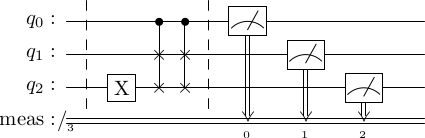
\includegraphics[scale = 0.5]{1a100.png}
        \subsection*{Output for input 100 is}
        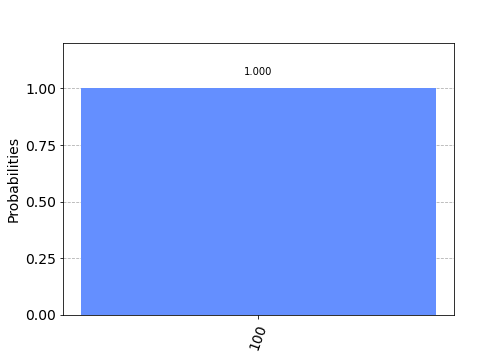
\includegraphics[scale = 0.5]{1a100-out.png}
        \subsection*{Circuit for 2 Fredkin gates on state 101}
        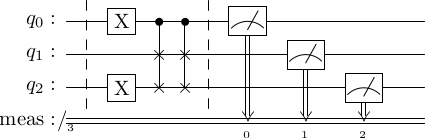
\includegraphics[scale = 0.5]{1a101.png}
        \subsection*{Output for input 101 is}
        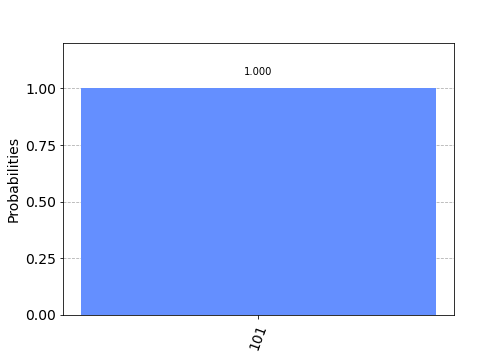
\includegraphics[scale = 0.5]{1a101-out.png}
        \subsection*{Circuit for 2 Fredkin gates on state 110}
        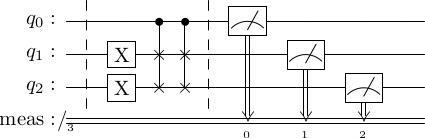
\includegraphics[scale = 0.5]{1a110.png}
        \subsection*{Output for input 110 is}
        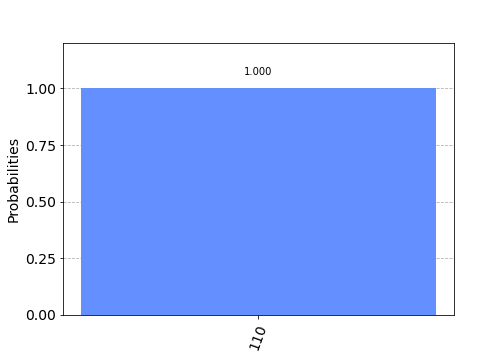
\includegraphics[scale = 0.5]{1a110-out.png}
        \subsection*{Circuit for 2 Fredkin gates on state 111}
        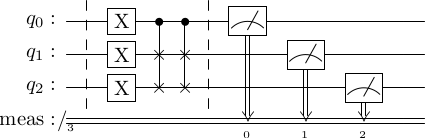
\includegraphics[scale = 0.5]{1a111.png}
        \subsection*{Output for input 111 is}
        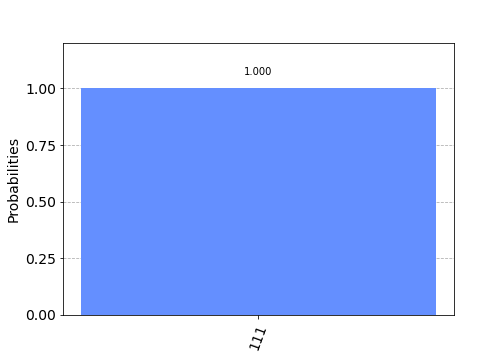
\includegraphics[scale = 0.5]{1a111-out.png}\\
        \begin{center}
            \begin{tabular}{ | m{3cm}| m{3cm} | } 
                \hline
                Input	&	Output \\
                \hline
                000 & 000\\
                001 & 001\\
                010 & 010\\
                011 & 011\\
                100 & 100\\
                101 & 101\\
                110 & 110\\
                111 & 111\\
                \hline
            \end{tabular}
        \end{center}
        Since, input is equal to output we can clearly say Fredkin gate is reversible gate. 
    \end{answer}
    \begin{answer}[Question 1 b (a)]
        \subsection*{LHS Circuit for input 00}
        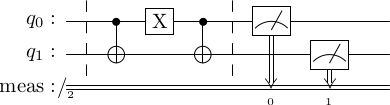
\includegraphics[scale=0.5]{a100.png}
        \subsection*{Output of LHS circuit for input 00}
        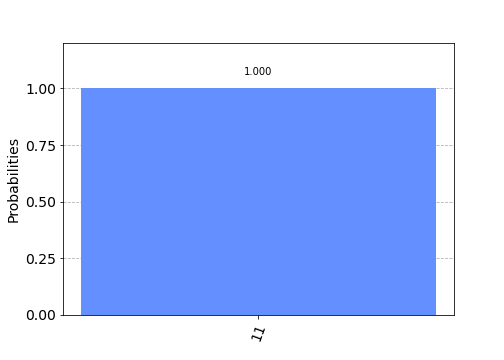
\includegraphics[scale = 0.5]{a100-out.png}
        \subsection*{RHS Circuit for input 00}
        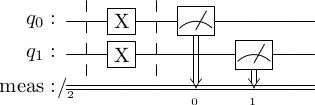
\includegraphics[scale=0.5]{a200.png}
        \subsection*{Output of RHS circuit for input 00}
        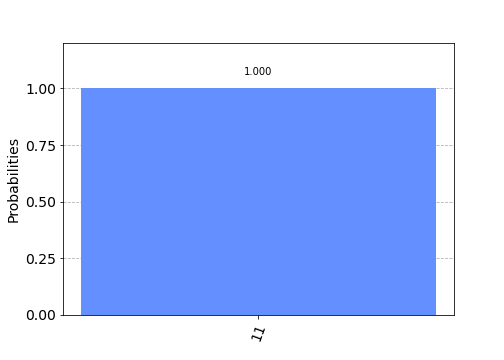
\includegraphics[scale = 0.5]{a200-out.png}
        \subsection*{LHS Circuit for input 01}
        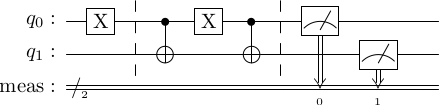
\includegraphics[scale=0.5]{a101.png}
        \subsection*{Output of LHS circuit for input 01}
        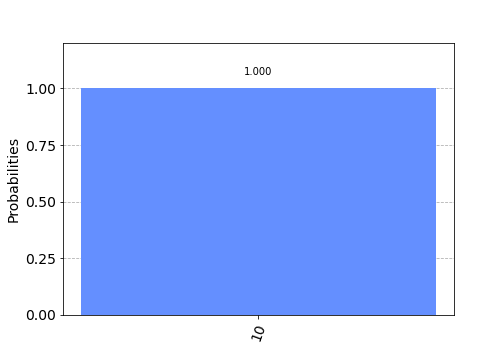
\includegraphics[scale = 0.5]{a101-out.png}
        \subsection*{RHS Circuit for input 01}
        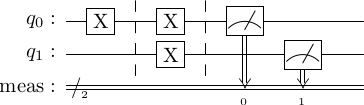
\includegraphics[scale=0.5]{a201.png}
        \subsection*{Output of RHS circuit for input 01}
        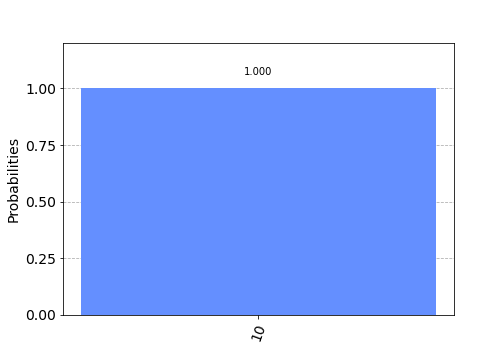
\includegraphics[scale = 0.5]{a201-out.png}
        \subsection*{LHS Circuit for input 10}
        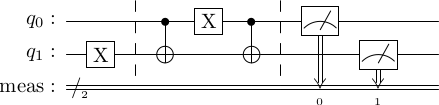
\includegraphics[scale=0.5]{a110.png}
        \subsection*{Output of LHS circuit for input 10}
        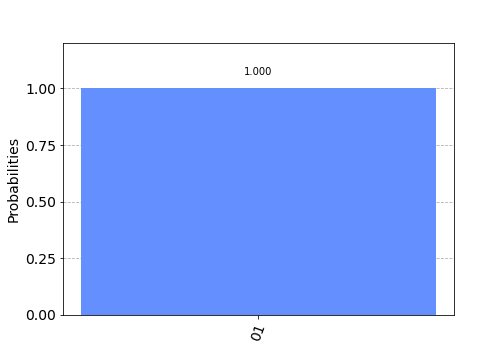
\includegraphics[scale = 0.5]{a110-out.png}
        \subsection*{RHS Circuit for input 10}
        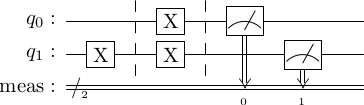
\includegraphics[scale=0.5]{a210.png}
        \subsection*{Output of RHS circuit for input 10}
        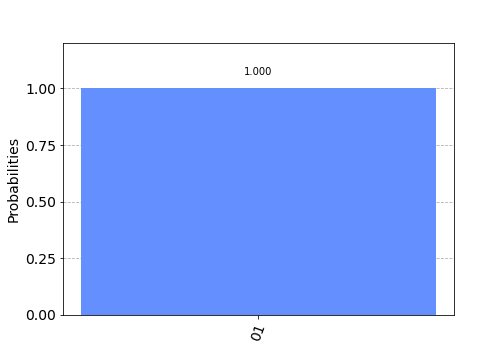
\includegraphics[scale = 0.5]{a210-out.png}
        \subsection*{LHS Circuit for input 11}
        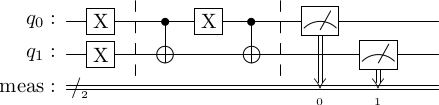
\includegraphics[scale=0.5]{a111.png}
        \subsection*{Output of LHS circuit for input 11}
        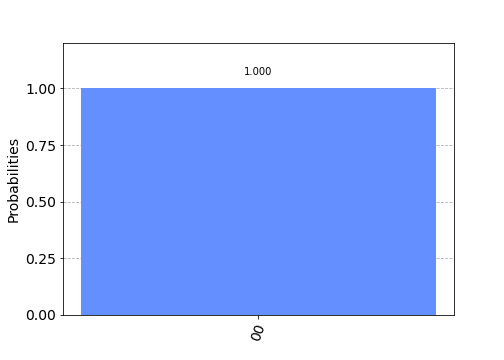
\includegraphics[scale = 0.5]{a111-out.png}
        \subsection*{RHS Circuit for input 11}
        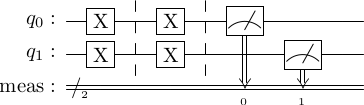
\includegraphics[scale=0.5]{a211.png}
        \subsection*{Output of RHS circuit for input 11}
        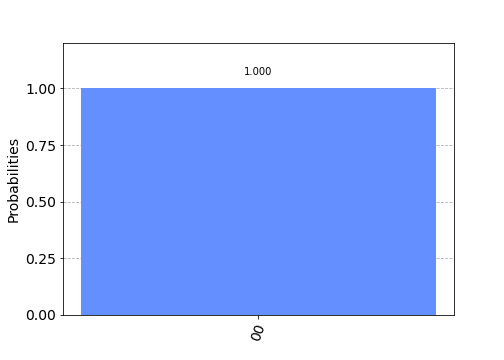
\includegraphics[scale = 0.5]{a211-out.png}\\
        Truth table        
        \begin{center}
            \begin{tabular}{ | m{3cm}| m{3cm} |m{3cm}| } 
                \hline
                Input	&	Output of LHS & Output of RHS \\
                \hline
                00 & 11&11\\
                01 & 10&10\\
                10 & 01&01\\
                11 & 00&00\\
                \hline
            \end{tabular}
        \end{center} 
        Since, truth table is same for both LHS and RHS both circuits are equivalent. 
    \end{answer}
    \begin{answer}[Question 1 b (b)]
        \subsection*{LHS Circuit for input 00}
        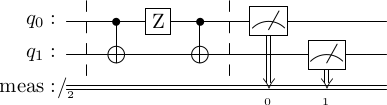
\includegraphics[scale=0.5]{b100.png}
        \subsection*{Output of LHS circuit for input 00}
        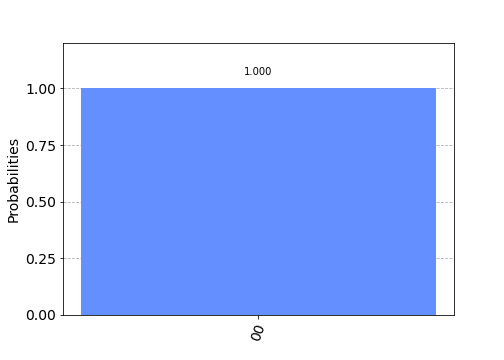
\includegraphics[scale = 0.5]{b100-out.png}
        \subsection*{RHS Circuit for input 00}
        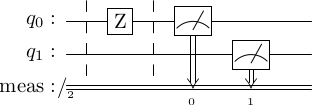
\includegraphics[scale=0.5]{b200.png}
        \subsection*{Output of RHS circuit for input 00}
        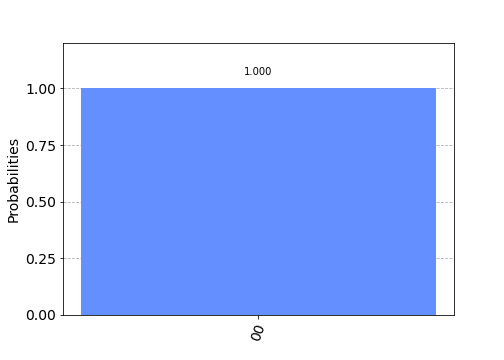
\includegraphics[scale = 0.5]{b200-out.png}
        \subsection*{LHS Circuit for input 01}
        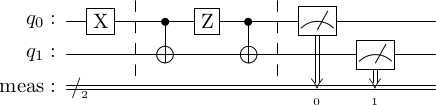
\includegraphics[scale=0.5]{b101.png}
        \subsection*{Output of LHS circuit for input 01}
        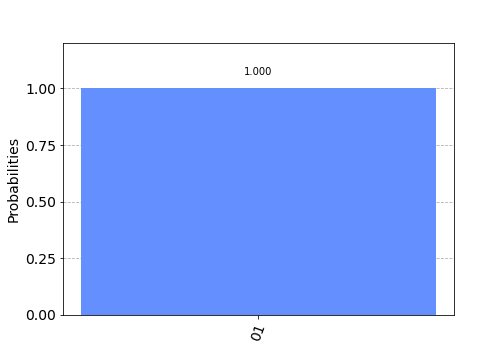
\includegraphics[scale = 0.5]{b101-out.png}
        \subsection*{RHS Circuit for input 01}
        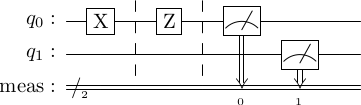
\includegraphics[scale=0.5]{b201.png}
        \subsection*{Output of RHS circuit for input 01}
        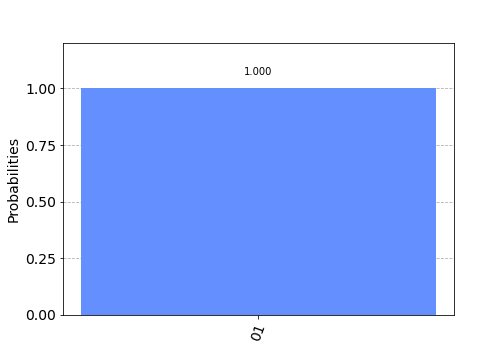
\includegraphics[scale = 0.5]{b201-out.png}
        \subsection*{LHS Circuit for input 10}
        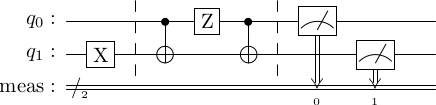
\includegraphics[scale=0.5]{b110.png}
        \subsection*{Output of LHS circuit for input 10}
        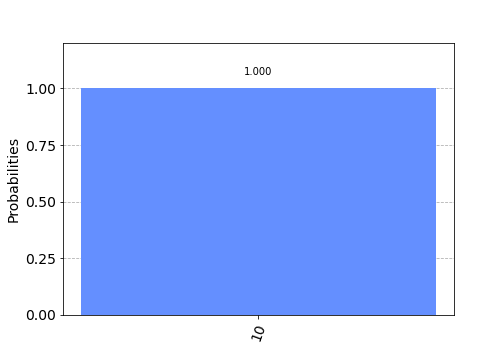
\includegraphics[scale = 0.5]{b110-out.png}
        \subsection*{RHS Circuit for input 10}
        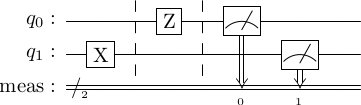
\includegraphics[scale=0.5]{b210.png}
        \subsection*{Output of RHS circuit for input 10}
        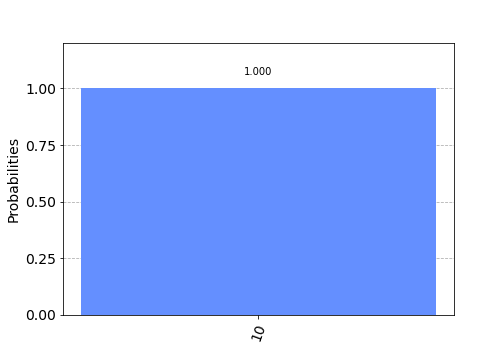
\includegraphics[scale = 0.5]{b210-out.png}
        \subsection*{LHS Circuit for input 11}
        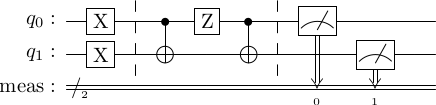
\includegraphics[scale=0.5]{b111.png}
        \subsection*{Output of LHS circuit for input 11}
        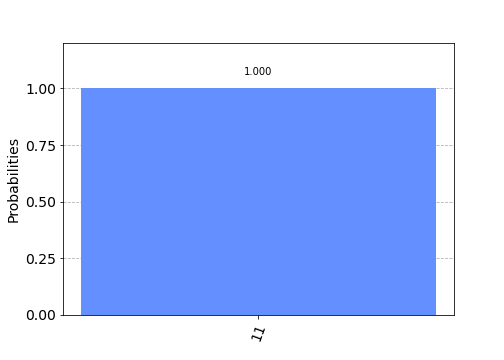
\includegraphics[scale = 0.5]{b111-out.png}
        \subsection*{RHS Circuit for input 11}
        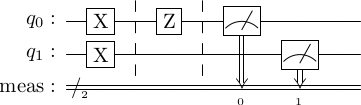
\includegraphics[scale=0.5]{b211.png}
        \subsection*{Output of RHS circuit for input 11}
        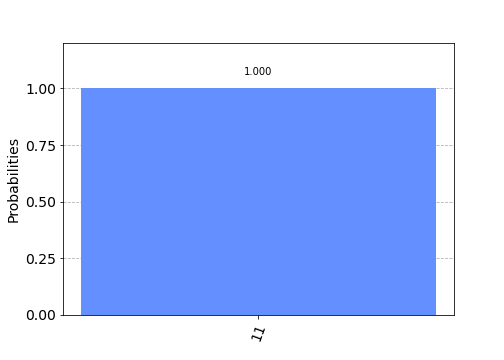
\includegraphics[scale = 0.5]{b211-out.png}
        Truth table        
        \begin{center}
            \begin{tabular}{ | m{3cm}| m{3cm} |m{3cm}| } 
                \hline
                Input	&	Output of LHS & Output of RHS \\
                \hline
                00 & 00&00\\
                01 & 01&01\\
                10 & 10&10\\
                11 & 11&11\\
                \hline
            \end{tabular}
        \end{center} 
        Since, truth table is same for both LHS and RHS both circuits are equivalent. 
    \end{answer}
    \begin{answer}[Qeusiton 1 b (c)]  
        \subsection*{LHS Circuit for input 00}
        \includegraphics[scale=0.5]{c100.png}
        \subsection*{Output of LHS circuit for input 00}
        \includegraphics[scale = 0.5]{c100-out.png}
        \subsection*{RHS Circuit for input 00}
        \includegraphics[scale=0.5]{c200.png}
        \subsection*{Output of RHS circuit for input 00}
        \includegraphics[scale = 0.5]{c200-out.png}
        \subsection*{LHS Circuit for input 01}
        \includegraphics[scale=0.5]{c101.png}
        \subsection*{Output of LHS circuit for input 01}
        \includegraphics[scale = 0.5]{c101-out.png}
        \subsection*{RHS Circuit for input 01}
        \includegraphics[scale=0.5]{c201.png}
        \subsection*{Output of RHS circuit for input 01}
        \includegraphics[scale = 0.5]{c201-out.png}
        \subsection*{LHS Circuit for input 10}
        \includegraphics[scale=0.5]{c110.png}
        \subsection*{Output of LHS circuit for input 10}
        \includegraphics[scale = 0.5]{c110-out.png}
        \subsection*{RHS Circuit for input 10}
        \includegraphics[scale=0.5]{c210.png}
        \subsection*{Output of RHS circuit for input 10}
        \includegraphics[scale = 0.5]{c210-out.png}
        \subsection*{LHS Circuit for input 11}
        \includegraphics[scale=0.5]{c111.png}
        \subsection*{Output of LHS circuit for input 11}
        \includegraphics[scale = 0.5]{c111-out.png}
        \subsection*{RHS Circuit for input 11}
        \includegraphics[scale=0.5]{c211.png}
        \subsection*{Output of RHS circuit for input 11}
        \includegraphics[scale = 0.5]{c211-out.png}
        Truth table        
        \begin{center}
            \begin{tabular}{ | m{3cm}| m{3cm} |m{3cm}| } 
                \hline
                Input	&	Output of LHS & Output of RHS \\
                \hline
                00 & 10&10\\
                01 & 11&11\\
                10 & 00&00\\
                11 & 01&01\\
                \hline
            \end{tabular}
        \end{center} 
        Since, truth table is same for both LHS and RHS both circuits are equivalent. 
    \end{answer}    
    \begin{answer}[Question 1 b (d)]
        \subsection*{LHS Circuit for input 00}
        \includegraphics[scale=0.5]{d100.png}
        \subsection*{Output of LHS circuit for input 00}
        \includegraphics[scale = 0.5]{d100-out.png}
        \subsection*{RHS Circuit for input 00}
        \includegraphics[scale=0.5]{d200.png}
        \subsection*{Output of RHS circuit for input 00}
        \includegraphics[scale = 0.5]{d200-out.png}
        \subsection*{LHS Circuit for input 01}
        \includegraphics[scale=0.5]{d101.png}
        \subsection*{Output of LHS circuit for input 01}
        \includegraphics[scale = 0.5]{d101-out.png}
        \subsection*{RHS Circuit for input 01}
        \includegraphics[scale=0.5]{d201.png}
        \subsection*{Output of RHS circuit for input 01}
        \includegraphics[scale = 0.5]{d201-out.png}
        \subsection*{LHS Circuit for input 10}
        \includegraphics[scale=0.5]{d110.png}
        \subsection*{Output of LHS circuit for input 10}
        \includegraphics[scale = 0.5]{d110-out.png}
        \subsection*{RHS Circuit for input 10}
        \includegraphics[scale=0.5]{d210.png}
        \subsection*{Output of RHS circuit for input 10}
        \includegraphics[scale = 0.5]{d210-out.png}
        \subsection*{LHS Circuit for input 11}
        \includegraphics[scale=0.5]{d111.png}
        \subsection*{Output of LHS circuit for input 11}
        \includegraphics[scale = 0.5]{d111-out.png}
        \subsection*{RHS Circuit for input 11}
        \includegraphics[scale=0.5]{d211.png}
        \subsection*{Output of RHS circuit for input 11}
        \includegraphics[scale = 0.5]{d211-out.png}
        Truth table        
        \begin{center}
            \begin{tabular}{ | m{3cm}| m{3cm} |m{3cm}| } 
                \hline
                Input	&	Output of LHS & Output of RHS \\
                \hline
                00 & 11&11\\
                01 & 10&10\\
                10 & 01&01\\
                11 & 00&00\\
                \hline
            \end{tabular}
        \end{center} 
        Since, truth table is same for both LHS and RHS both circuits are equivalent. 
        
    \end{answer}
    \begin{answer}[Question 2]
    \subsection*{Circuit for 3 qubit GHZ state}
       \includegraphics{ghz-3.png} 
    \subsection*{Output of IBMQ machine}
        \includegraphics[scale = 0.75]{w-3-out.png}
    \subsection*{Circuit for 4 qubit GHZ state}
        \includegraphics[scale=0.8]{ghz-4.png}
    \subsection*{Output of IBM Q machine for 4 - qubit GHZ state}
        \includegraphics[scale=0.6]{w-4-out.png}
    \subsection*{Circuit for 5 qubit GHZ state}
        \includegraphics[scale=0.6]{ghz-5.png}
    \subsection*{Output of IBM Q machine for 5 - qubit GHZ state}
        \includegraphics[scale=0.6]{w-5-out.png}
    \end{answer}
    \begin{answer}[Question 3 (a)]
        \begin{center}
            \begin{quantikz}[slice all]
                \lstick{qubit 0 \(\ket{0}\) }&\gate{H}&\ctrl{1}&\qw&\gate{X}&\qw\\
                \lstick{qubit 1 \(\ket{0}\) }&\qw   &\targ{}    &\ctrl{1} &\qw&\qw\\
                \lstick{qubit 2 \(\ket{0}\) }&\qw   &\qw        &\targ{}&\qw&\qw
            \end{quantikz}
        \end{center}
        Initial State,
        \begin{gather}
            \ket{\psi_0} = \ket{000}
        \end{gather}
        Applying Hadamard gate to qubit 0,
        \begin{gather}
            \ket{\psi_1} = \frac{1}{\sqrt{2} }(\ket{000}+\ket{001})
        \end{gather}
        CNOT gate with qubit 0 as control and qubit 1 as target,
        \begin{gather}
            \ket{\psi_2} = \frac{1}{\sqrt{2} }(\ket{000}+\ket{011})
        \end{gather}
        CNOT gate with qubit 1 as control and qubit 2 as target,
        \begin{gather}
            \ket{\psi_3} = \frac{1}{\sqrt{2} }(\ket{000}+\ket{111})
        \end{gather}
        Applying X gate on qubit 0,
        \begin{gather}
            \ket{\psi_4} = \frac{1}{\sqrt{2} }(\ket{001}+\ket{110})
        \end{gather}
    \end{answer}
    \begin{answer}[Question 3 (b)]
        \begin{center}
            \begin{quantikz}[slice all]
                \lstick{qubit 0 \(\ket{0}\) }&\gate{H}&\ctrl{1}&\qw&\qw&\qw\\
                \lstick{qubit 1 \(\ket{0}\) }&\qw   &\targ{}    &\ctrl{1} &\gate{X}&\qw\\
                \lstick{qubit 2 \(\ket{0}\) }&\qw   &\qw        &\targ{}&\qw&\qw
            \end{quantikz}
        \end{center}
        Initial State,
        \begin{gather}
            \ket{\psi_0} = \ket{000}
        \end{gather}
        Applying Hadamard gate to qubit 0,
        \begin{gather}
            \ket{\psi_1} = \frac{1}{\sqrt{2} }(\ket{000}+\ket{001})
        \end{gather}
        CNOT gate with qubit 0 as control and qubit 1 as target,
        \begin{gather}
            \ket{\psi_2} = \frac{1}{\sqrt{2} }(\ket{000}+\ket{011})
        \end{gather}
        CNOT gate with qubit 1 as control and qubit 2 as target,
        \begin{gather}
            \ket{\psi_3} = \frac{1}{\sqrt{2} }(\ket{000}+\ket{111})
        \end{gather}
        Applying X gate on qubit 1,
        \begin{gather}
            \ket{\psi_4} = \frac{1}{\sqrt{2} }(\ket{010}+\ket{101})
        \end{gather}
    \end{answer}
    \begin{answer}[Question 3 (c)]
        \begin{center}
            \begin{quantikz}[slice all]
                \lstick{qubit 0 \(\ket{0}\) }&\gate{H}&\ctrl{1}&\qw&\qw&\qw\\
                \lstick{qubit 1 \(\ket{0}\) }&\qw   &\targ{}    &\ctrl{1} &\qw&\qw\\
                \lstick{qubit 2 \(\ket{0}\) }&\qw   &\qw        &\targ{}&\gate{X}&\qw
            \end{quantikz}
        \end{center}
        Initial State,
        \begin{gather}
            \ket{\psi_0} = \ket{000}
        \end{gather}
        Applying Hadamard gate to qubit 0,
        \begin{gather}
            \ket{\psi_1} = \frac{1}{\sqrt{2} }(\ket{000}+\ket{001})
        \end{gather}
        CNOT gate with qubit 0 as control and qubit 1 as target,
        \begin{gather}
            \ket{\psi_2} = \frac{1}{\sqrt{2} }(\ket{000}+\ket{011})
        \end{gather}
        CNOT gate with qubit 1 as control and qubit 2 as target,
        \begin{gather}
            \ket{\psi_3} = \frac{1}{\sqrt{2} }(\ket{000}+\ket{111})
        \end{gather}
        Applying X gate on qubit 2,
        \begin{gather}
            \ket{\psi_4} = \frac{1}{\sqrt{2} }(\ket{100}+\ket{011})
        \end{gather}
    \end{answer}
    \begin{answer}[Question 4]
        \subsection*{Circuit for W-state}
        \includegraphics[scale = 0.6]{w-4-state.png}
        \subsection*{State tomography}
        \includegraphics[scale = 0.3]{tomography.png}
        \[
            \boxed{\text{ Entangled bipartite states }: \frac{1}{2}(\ket{0001}+\ket{0010}+\ket{0100}+\ket{1000})}
        \]
    \end{answer}
    \begin{answer}[Question 5 a]
        Construction of a N - Qubit GHZ gate
        \begin{verbatim}
            N = int(input('Please enter no.of Qubits')) 
                                => Number of qubits can be manually entered 
            qc = QuantumCircuit(N) => Making a quantum circuit of with N qubits. 
            qc.h(0) => Applying Hadamard gate to zeroth qubit.
            for i in range(1,N):
                qc.cx(i-1,i) => CNOT gate is applied to every qubit as target
                                qubit and previous one as control qubit
            qc.measure_all()
            qc.draw()
        \end{verbatim}
        \subsection*{A 4 qubit GHZ gate}
        \includegraphics[scale = 0.7]{5a.png}
    \end{answer}
    \begin{answer}[Question 5 b]
        Construction of a N - Qubit Entangled bipartite state 
        \begin{verbatim}
            N=int(input('Please enter no.of Qubits'))
                            => Number of qubits can be manually entered 
            qc = QuantumCircuit(N) => Making a quantum circuit of with N qubits.
            qc.ry(2*np.arccos(1/np.sqrt(N)),0) 
                    => Qubit 0 is Rotated 2arccos(1/sqrt(N)) times w.r.t y-axis 
            for i in range(1,N):
                qc.cry(2*np.arccos(1/np.sqrt(N-i)),i-1,i)
                    => Qubit i is target qubit rotated 2arccos(1/sqrt(N-i)) 
                        times w.r.t y-axis and i-1 qubit is control qubit 

            for i in range(1,N):
                qc.cx(N-i-1,N-i) => CNOT gate is applied on i th qubit 
                                    with i-1 th qubit as control qubit. 
            qc.x(0)=> NOT gate is applied on qubit 0. 
            qc.draw()
        \end{verbatim}
        \subsection*{A 5 qubit Entangled bipartite state}
        \includegraphics[scale = 0.6]{5-b.png}
    \end{answer}
\end{document}
